This thesis focuses in the efficient numerical solution of parametrized unsteady PDEs with moving meshes.

Parametrized PDEs can be numerically solved with the finite element method (FEM), 
which leads to an algebraic system of equations whose solution 
can be computationally expensive to obtain, 
especially for complex geometries or elaborate models.
One refers to this FEM model as the \textit{Full Order Model}~(FOM),
\begin{equation}
   \frac{du_h}{dt} + A_h\left(t;\mu\right) u_h = f_h\left(t;\mu\right).
\end{equation}
When the problem is unsteady, that is, 
when the differential operators contain terms that change in time,
or the mesh moves in time (effectively changing the integrals of the weak form),
the algebraic operators need to be reassembled for each timestep.

When this is the case, many-query procedures and access to field values or 
calculated outputs for different parameter values $\mu$ can become cumbersome, 
or even infeasible due to computational costs, both in time and memory.
To circumvent the efficiency issues, one can build a \textit{Reduced Order Model}~(ROM), 
whose solution is fast in time and light in storage.
This ROM is based in ad-hoc empirical basis functions to represent the solution, 
whose support typically spans the whole domain. 

However, due to the change in time of the operators, 
using a standalone reduced basis to represent the solution
is not enough to remove all the overheads of the FEM model.
The operators still need to be assembled 
and projected in the reduced space for each timestep.
The reduced basis of the solution does shrunk the overall dimension of the system,
but it cannot remove the overhead derived from the inevitable change in the operators.
We would state to have an \textit{offline-online coupling},
since information from the FOM is required to assemble the ROM.
To overcome this issue, a system approximation technique is introduced.
We then talk about an \textit{Hyper Reduced Order Model}~(HROM).

\subsection{Outline of the Reduction Process}
The construction of the ROM has mainly two stages:
\begin{itemize}
   \item Offline stage: construction of the ROM ingredients.
   \item Online stage: assembly of the ROM to solve the PDE for unseen parametrizations.
\end{itemize}

During the offline stage, the costly algebraic problem is solved for a subset of the parameter space.
Snapshots of the matrices, vectors and solutions are stored and processed via algebraic reduction algorithms, 
in order to obtain a reduced basis for each of them.

An example of reduction algorithms would be the Discrete Empirical Interpolation Method (DEIM) 
and its matrix version (MDEIM).
These reduction algorithms need to rely on a procedure to construct the basis, 
in our case we will use the Proper Orthogonal Decomposition (POD). 

The offline stage scales with the dimension of the Full Order Model, $N_h$, 
which is governed by the number of nodes in the mesh and the polynomial degree for the FEM basis.
Once the offline stage is over, a basis for each operator of the algebraic problem has been produced, 
of representative\footnote{
   The reduction of each operator might have required a different number of basis elements, 
   but they should be all of the same order of magnitude $N \ll N_h$ or smaller for the reduction process to be a success.}
size~$N \ll N_h$.
A projection matrix $\mathbb{V}$ is derived from the solution reduced basis, 
\begin{equation}
   \mathbb{V} \in \mathbb{R}^{N_h \,\text{x}\, N}.
\end{equation} 
This matrix will be used to project once and for all 
the algebraic operator reduced basis elements, 
our HROM building blocks.
The reduced bases for the solution and the algebraic operators 
are then used during the online stage, 
where for unseen parameters a small algebraic system is built and solved,
\begin{equation}
   \frac{du_N}{dt} + A_N\left(t;\mu\right) u_N = f_N\left(t;\mu\right).
\end{equation}
At this stage, it is paramount that the assembly of the operators\footnote{
   We shall overload notation and refer to \textit{the operator} for both the matrices and the functionals,
   unless explicit distinction is required.
} 
is independent of the original problem size $N_h$.
We state to have a perfect \textit{offline-online decoupling}.

Once the reduced problem has been solved, the solution can be projected back to the original physical mesh,
\begin{equation}
   u_h = \mathbb{V} u_N.
\end{equation}
Following these steps, access to field values or calculated outputs can be obtained lightly, 
provided the overall procedure is \textit{certified}: 
to prove in the online stage that the solution is sufficiently close 
to what it would have been if the actual FOM had been assembled and solved.

All the above is presented graphically in Figure~\ref{fig:overview_graph}.

\subsection{System Approximation}
An essential ingredient to achieve a perfect \mbox{offline-online} decoupling
is what we call an \textit{
   affine decomposition} 
of the algebraic operators.
Simply put, it is to say that we can achieve a linear separation 
in the parameter, time, and spatial domains 
(the latter represented by the algebraic basis elements), 
\begin{equation}
   A_h\left(t;\mu\right) = \sum_{q=1}^{Q} \Theta_{q}(t;\mu) A_{h,q},
\end{equation}
where~$A_{h,q}$ are constant matrices referred to as the collateral basis,
and~$\Theta_{q}(t;\mu) \in \mathbb{R}$ are scalar values. 

The easiest example one could come up with of an affine decomposition is the one present 
in the heat diffusion problem with two different but uniform diffusion parameters $k_q$ across the domain.
The affine decomposition would look like
\begin{equation}
   A_h\left(t;k_1, k_2\right) = k_{1} A_{h,1} + k_{2} A_{h,2},
\end{equation}
where each matrix $A_{h,q}$ would represent the diffusion operator with support over the subdomain associated with each parameter. 
For this simple example, the affine decomposition is present naturally within the PDE structure, 
but this will not always be the case, specially when nonlinearities are present. 

However, nowadays it is absolutely possible to obtain an automatic ad-hoc affine decomposition 
for any operator thanks to grounded algorithms and procedures, like DEIM and MDEIM.
This key fact will allows us to achieve a perfect split between the offline and the online stage, 
as it will allow us to assemble our ROM operators without having to assemble at any point the complete FOM operator. 

\subsubsection{Nonlinear Term Reduction}
The reduction of a nonlinear term can be achieved 
with the same MDEIM technique as the one used for linear operators.

The only difference is that the coefficient functions~$\Theta_{q}$ from 
the affine decomposition depend on the solution values too,
\begin{equation}
   A_h\left(t;\mu\right, u) = \sum_{q=1}^{Q} \Theta_{q}(t;\mu, u) A_{h,q}.
\end{equation}
Nevertheless, this fact does not necessarily break the convergence and approximation 
properties derived for MDEIM,
so we expect to use it successfully.   

% Ideally, 
%% Research objectives
% Useful: benefit of your research to the problem. 
% Realistic: contribute to the solution of the problem.
% Feasible: time scheduled and capabilities and resources.
% Clear: be precise in the contribution to the problem.
% Informative: rough idea of knowledge generated towards a solution.

% The research objective is (a) by (b).
% (a) The contribution of the research project to the solution of the problem.
% (b) description of the way the contribution will be provided. 

\subsubsection{Implicit \textit{Nonlinearities}}
A nonlinearity can be seen essentially as a characteristic that prevents a linear separation.
Despite the apparent linear character of an algebraic equation, 
from the point of view of the affine decomposition, 
it could potentially hide a nonlinearity.

The introduction of the time variable~$t$~in the shape of the mesh makes it so
that the operators change at each time step during the integration loop.
Additionally, since the domain geometry will depend on some parameter values too, 
one cannot explicitly write the affine decomposition of the operators in a closed form.
This is implicitly collected by the Jacobian,
the transformation that maps integrals over moving meshes 
to one over a reference fixed mesh.

Another type of nonlinearity would be a term whose integrand contained 
a nonlinear function applied over the $u$ field,
or interactions of the solution with its own derivatives.
% These kind of non-linearities are common in mathematical modelling, 
% but shall keep out of the scope of this work to keep a narrow focus. 
% The non-linearity of the basic operators will give us enough work already.

\subsection{Kick-off Point}
The (M)DEIM reduction technique have been successfully used with domains
whose boundary is parametrized, but whose mesh remained fixed in time \cite{Santo_Manzoni_2019}. 

We aim at extending these results by introducing a moving mesh in time,
thus allowing us to obtain an hyper reduced order model which can tackle 
more complex \mbox{real-life} problems.
The additional complexities introduced by the moving mesh are the introduction 
of the Arbitrary Eulerian Lagrangian formulation (ALE), 
and the increase in the number of operator snapshots to be collected during the offline stage.  

\onecolumn
\begin{figure}[h]
   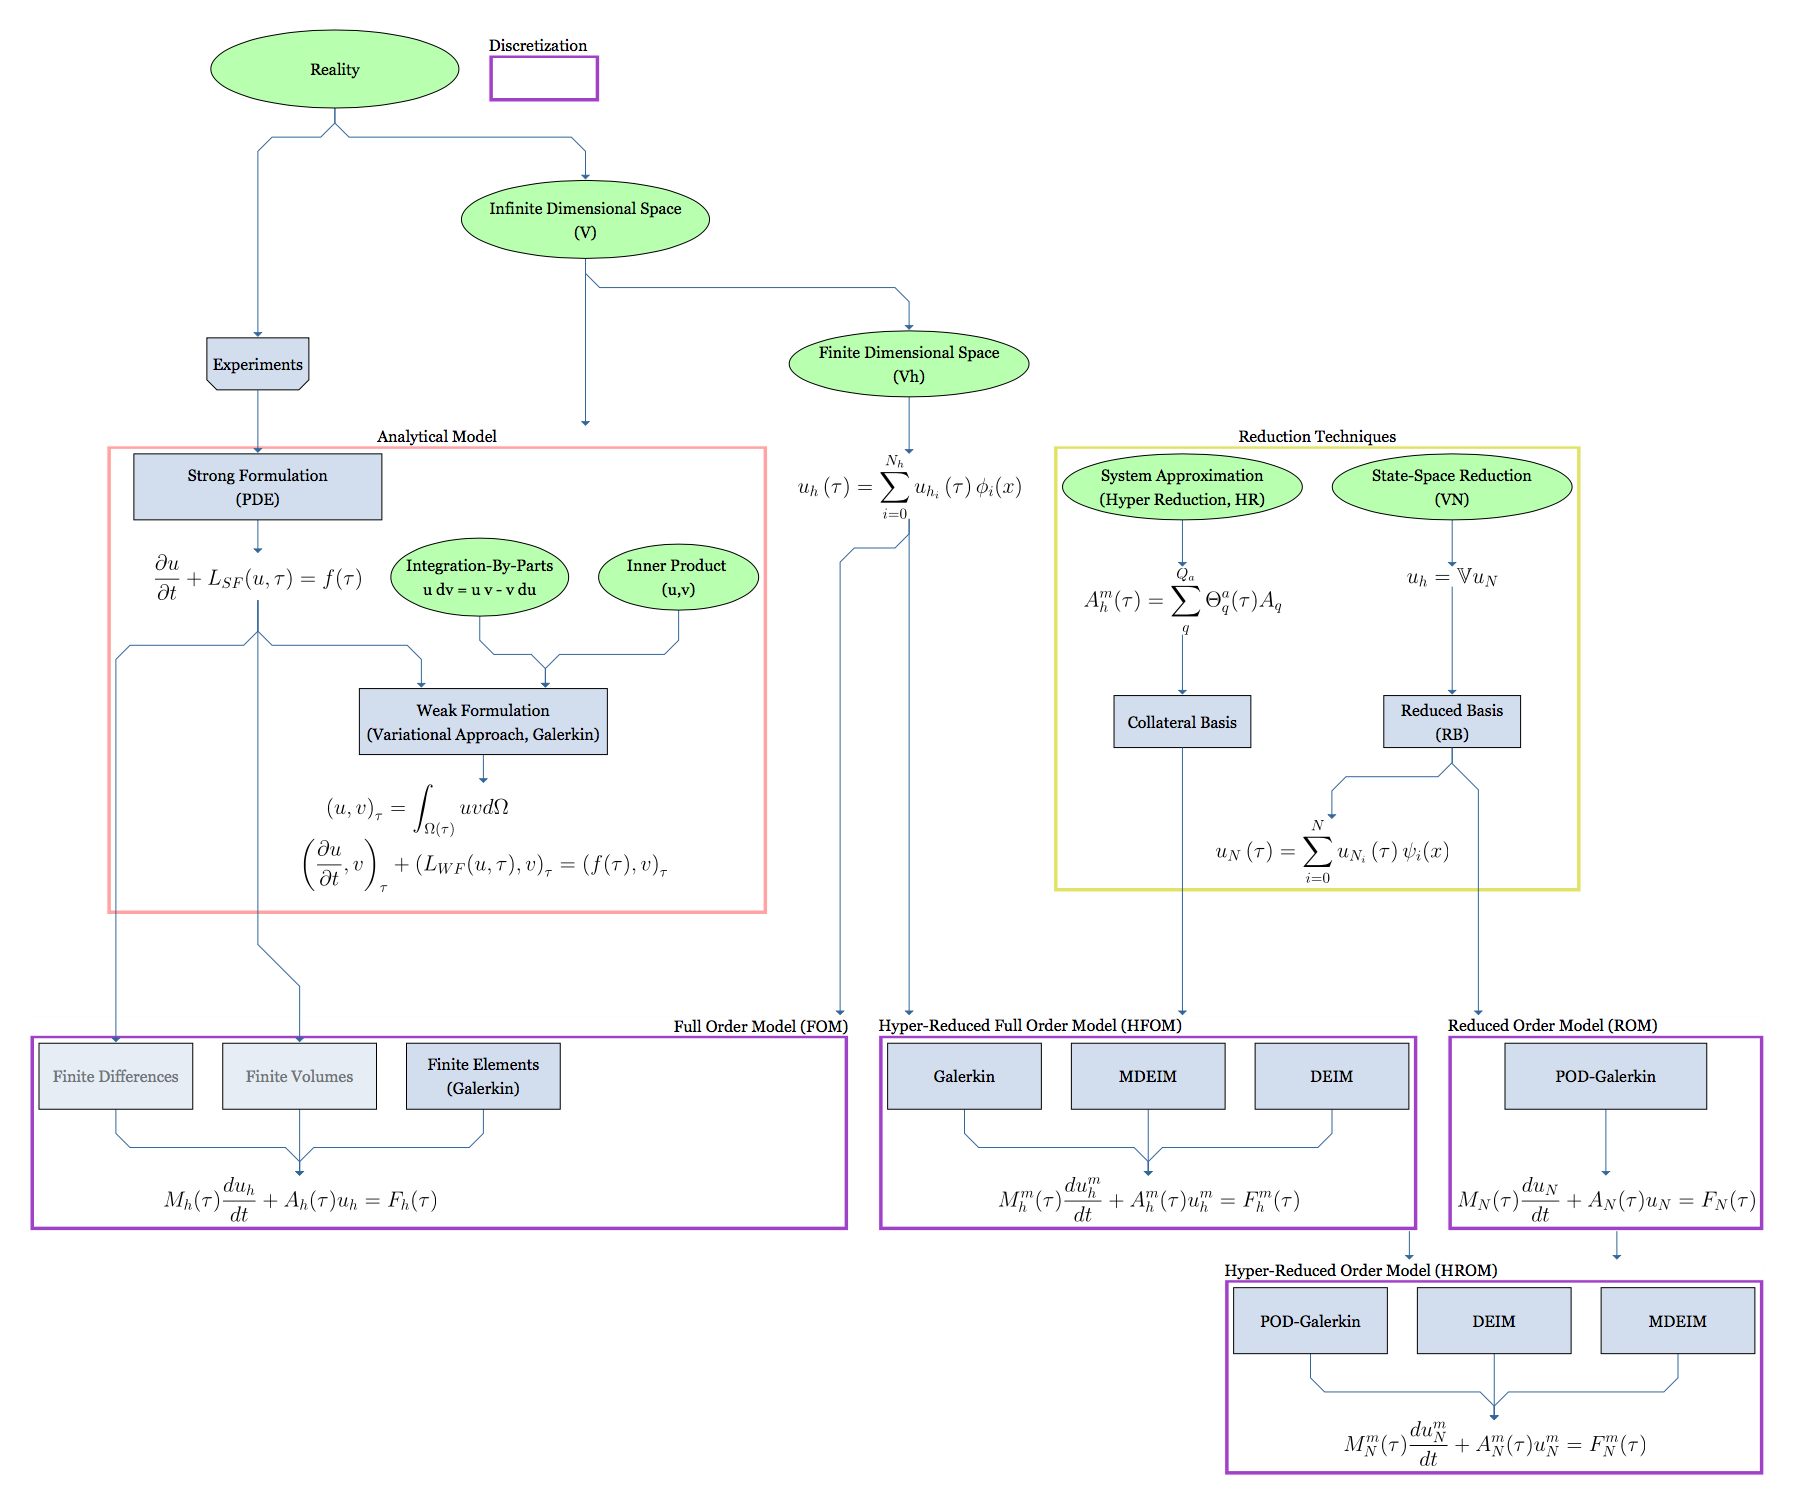
\includegraphics[width=\columnwidth]{graphs/From-Reality-To-ROM.png}
   \caption{Building blocks of the transition from reality to discrete 
   reduced order modeling.
   On the left side we present the traditional finite element course: 
   from the observation of reality a parametrized PDE model is derived 
   (infinite dimensional space, unknown analytical solution).
   The paremeters allow the model to capture a range of 
   boundary conditions, geometries,
   and term-domination effects, 
   all of them driven by the same physics.
   % 
   This model can be cast into a weak form and 
   solved numerically via the Galerkin projection 
   (finite dimensional space, Lagrangian piecewise solution).
   The finite element method is a robust and well-established technique
   for the solution of parametrized PDEs.
   However, for three-dimensional domains, 
   or complex modelling terms, the algebraic operators involved (vectors and matrices) 
   can become computationally expensive to assemble and solve,
   especially for unsteady problems with moving meshes.
   % 
   On the right side, we present two reduction techniques introduced 
   to increase the efficiency of the numerical solution:
   the construction of a \textit{reduced basis} (RB), also known as state-space reduction;
   and the determination of a collateral basis for 
   the algebraic finite element operators, known as \textit{system approximation}.
   The reduced basis is used in substitution of the Lagrangian piecewise functions,
   the collateral basis is used to skip the assembly 
   of all the entries of each algebraic operator.
   % 
   All in all, the simultaneous use of these two reduction techniques 
   leads to an algebraic hyper-reduced order model,
   cheaper to assemble and solve than the traditional finite element problem;
   and for problems with time-dependent matrices,
   even cheaper than assembling the operators and projecting them
   unto the reduced basis for each timestep.}
   \label{fig:overview_graph}
 \end{figure}
 \twocolumn